\documentclass[10pt,twocolumn,letterpaper]{article}

\usepackage{cvpr}
\usepackage{times}
\usepackage{epsfig}
\usepackage{graphicx}
\usepackage{amsmath}
\usepackage{amssymb}
\usepackage{multirow}
\usepackage{graphicx}

% Include other packages here, before hyperref.

% If you comment hyperref and then uncomment it, you should delete
% egpaper.aux before re-running latex.  (Or just hit 'q' on the first latex
% run, let it finish, and you should be clear).
\usepackage[pagebackref=true,breaklinks=true,letterpaper=true,colorlinks,bookmarks=false]{hyperref}

% \cvprfinalcopy % *** Uncomment this line for the final submission

\def\cvprPaperID{****} % *** Enter the CVPR Paper ID here
\def\httilde{\mbox{\tt\raisebox{-.5ex}{\symbol{126}}}}

% Pages are numbered in submission mode, and unnumbered in camera-ready
\ifcvprfinal\pagestyle{empty}\fi
\begin{document}

%%%%%%%%% TITLE
\title{Bi-Directional Domain Translation for Zero-Shot Sketch-Based Image Retrieval}

\author{First Author\\
Institution1\\
Institution1 address\\
{\tt\small firstauthor@i1.org}
% For a paper whose authors are all at the same institution,
% omit the following lines up until the closing ``}''.
% Additional authors and addresses can be added with ``\and'',
% just like the second author.
% To save space, use either the email address or home page, not both
\and
Second Author\\
Institution2\\
First line of institution2 address\\
{\tt\small secondauthor@i2.org}
}

\maketitle
%\thispagestyle{empty}

\maketitle
%\thispagestyle{empty}

%%%%%%%%% ABSTRACT
\begin{abstract}
   %Zero-shot sketch-based image retrieval (ZS-SBIR) is a cross-modal retrieval task, which use free-hand sketches to retrieve from natural image gallery where test categories do not appear at training stage. However, previous works rely on either aligned data pairs to reduce gap between seen and unseen categories or semantic information to reduce the intra-class variance, which need extra data and cannot perform structure-based retrieval. In contrast, we propose to use disentangled representation to train a structure-based model. 
   %First sentence introduces SBIR 
   %Second sentence introduces zero-shot SBIR.
   %Third sentence: traditional SBIR method are prone to be class-based retrieval and cannot generalized well to unseen categories. 
   %Fourth sentence: In contrast, we disentangle image feature into structure feature and appearance feature to facilitate structure-based retrieval.  
   Sketch-Based Image Retrieval (SBIR) is cross-modal retrieval task, which use free-hand sketches to retrieve from natural image gallery with the \textbf{same category}. 
   However, SBIR requires all categories can be seen during training, which is not guaranteed. 
   So we investigate a more challenging task, Zero-Shot Sketch-Based Image Retrieval (ZS-SBIR), in which testing categories do not appear in the training stage. 
   Traditional SBIR method are prone to be class-based retrieval and cannot generalize well from seen categories to unseen ones. 
   In contrast, we disentangle image feature into structure feature and appearance feature to facilitate structure-based retrieval.
   To realize the function of feature disentanglement and take full advantage of disentangled information, we propose Bi-directional Domain Translation for zero-shot sketch-based image retrieval (BDT) framework, in which the image domain and sketch domain can be translated to each other through disentangled structure and appearance feature.
   Moreover, we also perform retrieval in both structure feature space and image feature space. 
   Extensive experiments demonstrate that our proposed approach remarkably outperforms state-of-the-art approaches by more than 8\% on Sketchy dataset and about 5\% on TU-Berlin dataset in the retrieval.
\end{abstract}

%%%%%%%%% BODY TEXT
\section{Introduction}

% First Edition
%In recent year, with the rapid growth of multimedia data on the internet, the role of image retrieval has become more and more important in many fields, such as remote sensing and e-commerce. Since the sketch can be easily drawn and express shape and pose details about the target images, sketch-based image retrieval (SBIR) has become widely accepted among users. Therefore, SBIR has also attracted widespread attention in the research community \cite{del1997visual, cao2010mindfinder, eitz2010evaluation, eitz2010sketch, cao2011edgel, hu2011bag, zhou2012sketch, hu2013performance, cao2013sym, saavedra2014sketch, parui2014similarity, james2014reenact, wang2015sketch, saavedra2015sketch, li2016fine, yu2016sketch, qi2016sketch, sangkloy2016sketchy, lu2018learning}. Since, all the above works are based on a hypothesis that all the categories for both image and sketch are known, in which setup existing approaches achieved satisfying performance \cite{lu2018learning}. However, in realistic situation, this hypothesis may not stand.

%In this paper, we investigate a more challenge setup called zero-shot sketch-based image retrieval (ZS-SBIR), which assure that the test categories do not appear at training stage. And the goal of this setting is to adopt the model's generalization from known domain to unknown domain. Extensive experiments show that the performance of existing methods will decline rapidly at ZS-SBIR \cite{yelamarthi2018zero} setup mainly because of the large intra-class variance of sketch and the over-fitting problem in known domain.

%Due to some characteristics of sketches and the zero-shot setup, ZS-SBIR is extremely challenging. Specifically, (1) the sketches are visually sparsity and have large intra-class variance, since the sketches are only an outline of an object and different people tend to draw sketches with varied levels of abstraction (2) the zero-shot setup requires the model being capable of generalizing from known domain towards unknown domain.

%To tackle these problems, there are two kinds of solutions. For the first kind of works, they adopt generative model and use the sketch features to reconstruct the image features \cite{yelamarthi2018zero, wang2019stacked, xu2019semantic}. And for the second kind of works, they map the image features and sketch features into a shared feature space using the same or different feature extractor(s) \cite{shen2018zero, dutta2019semantically, liu2019semantic}. The difference among them mainly locates on how to use the extra information, like pre-trained word vector or WordNet, more properly. Both of them only use part of the cross-modal domain knowledge and try to use the extra information to increase the capability of transferring knowledge from the seen domain to the unseen domain.

%Different from these two kinds of methods, we propose an asymmetric unified bi-directional domain translation framework according to the difference characteristics of sketch and image, to combine the best of both kind of methods. In detail, the sketch only contain an outline of the image, which we define as structure information whereas the image also contains extra detailed information such as background and color, which we define as appearance information. Based on the characteristics of images and sketches we adopt two image encoder and an orthogonal loss to disentangle the image feature into structure features and appearance features and one sketch encoder to map the sketch feature into a shared space with image structure features. During decoding, a variational decoder is adopted to combine the image appearance information and the sketch information together to not only compensate the uncertainty during generating the image features but also facilitate the inference process. Moreover, to combine the best of the above two methods, we design a new retrieval strategy to combine the shared feature space and image feature space. The overall model and the new retrieval strategy is verified by the quantitative experimental results. 

%Our main contributions of this paper are summarized as follows:
%\begin{itemize}
%	\item An asymmetric unified bi-directional domain translation framework is designed for zero-shot sketch-based image retrieval. With two image encoder and a variational decoder, our model is capable of mapping the image features and sketch features into a shared space, and mapping the sketch feature into image space at the same time.
%	\item For the facilitate of using the information from both shared domain mapping and image domain reconstruction, we design a new retrieval strategy to combine the best of the two methods.
%	\item Experimental results on two popular large-scale datasets show that our approach significantly outperforms state-of-the-art methods in terms of retrieval performance.
%\end{itemize}


%% 1. 多媒体的发展是的image retrieval的主要动力
%% 2. sketch中蕴含着image的形状和形态信息,且容易绘画,所以渐渐变成一个研究热点
%% 3. 传统的设置,假设训练集合和测试集合所拥有的模型是相同的,所以主要关注如何减小sketch的intra-class variance和如何有效利用sketch中的稀疏的信息。经过多年的发展,sbir也取得了很好的效果。
%% 4. 但是这种假设在实际中不存在!
In recent years, with the rapid growth of multimedia data on the internet, the role of image retrieval has become more and more important in many fields, such as remote sensing and e-commerce. 
Since the sketch can be easily drawn and express structure and pose details about the target images, sketch-based image retrieval (SBIR), which use a sketch to retrieve images with the same category, has become widely accepted among users. 
Therefore, SBIR has also attracted widespread attention in the research community \cite{del1997visual, cao2010mindfinder, eitz2010evaluation, eitz2010sketch, cao2011edgel, hu2011bag, zhou2012sketch, hu2013performance, cao2013sym, saavedra2014sketch, parui2014similarity, james2014reenact, wang2015sketch, saavedra2015sketch, li2016fine, yu2016sketch, qi2016sketch, sangkloy2016sketchy, lu2018learning}. 
In the conventional setting, it is assumed that the images and sketches in training and testing set share the same categories.
However, in real-world applications, the categories of test sketches/images may be out of the scope of training categories.

%% 1. 本文主要研究zero-shot情况下的这一问题
%% 2. 前人的研究已经证明,在这种情况下,传统的模型并不能取得很好的效果,这主要是因为因为评价指标的导向会使得模型更加倾向于学习基于类别的检索方式,而这种情况并不存在于zero-shot的情况下。
%% 3. zs情况下主要的的问题是如何提升将模型从seen domain泛化到unseen domain。
In this paper, we investigate a more challenge task called zero-shot sketch-based image retrieval (ZS-SBIR), which assure that the test categories do not appear at training stage. 
It has been shown that the performance of existing methods will decline dramatically at ZS-SBIR setup \cite{yelamarthi2018zero} probably probably because they prone to learn category-based retrieval.
Specifically, since the evaluation methodology is category-based, traditional SBIR methods may take a shortcut by correlating sketches/images with their category labels and retrieving the images from the same category as the query sketch \cite{yelamarthi2018zero} which is very effective when testing data share the same category as training data. 
However, they often fail when the testing categories have never been seen in the training stage.
%Current evaluation methodology \cite{sangkloy2016sketchy} focuses only on category-based retrieval and the sketch-image pairs are generated based on whether they belong to the same category during train, both of which make the model prone to learning category-based retrieval. Therefore, it is hard for traditional SBIR methods to generalize from seen categories to unseen categories.  
% As most of the zero-shot tasks, the ZS-SBIR is extremely challenging, because it requires model being capable of transferring visual representation from seen domain to unseen domain and reduce the intra-class variance in sketch at the same time.

%% 1. 为了解决这个问题,一些人尝试使用生成式模型和pose对应的数据来增强模型在seen和unseen domain之间的泛化能力; 一些人尝试使用semantics信息来减小sketch的intra-class bias; 一些人尝试使用semantics的信息来引导同类别sketch和image的correspondence或保留预训练模型中的关键信息。; 
%% 2. 但是pose对应的数据并不容易得到,同时使用semantics信息也难以使得模型的脱离class-based retrieval.(第二点理由应该再重新组织一下)
%% 3. 与他们不同,我们打算将模型的变为倾向于基于结构特征的检索模型。
%% 1) traditional SBIR methods are prone to be class-based retrieval, so these methods cannot generalize to unseen categories. 
%% 2) To generalize well to unseen categories, structure-based retrieval is preferred.
%% 3) Existing zero-shot SBIR XXXXX (categorize and introduce their methods). However, they did not achieve the goal of structure-based retrieval.
%% 4) In this paper, we disentangle structure feature from image feature to facilitate structure-based retrieval. 
To generalize well from seen categories to unseen categories, a model should learn to align  the structure information of sketches with the corresponding structure information of images, which is referred to as structure-based retrieval.  
%Typically, there are two types of image-sketch pair, aligned pair and unaligned pair. The first type requires the image and sketch have same shape and pose and the second type only require the sketch and image belong to the same category.
Existing methods for ZS-SBIR can be categorized into three groups, 
(1) some works use generative model based on aligned data pairs, where image and sketch have same shape and pose, to reduce the gap between seen and unseen categories \cite{yelamarthi2018zero}; 
(2) some works use semantic information to reduce the intra-class variance in sketch to stabilize the training process \cite{xu2019semantic, wang2019stacked, dutta2019semantically, shen2018zero}; 
(3) some works fine-tune the pre-trained model in ZS-SBIR task, with semantic-aware knowledge preservation to prevent catastrophic forgetting \cite{liu2019semantic}. 
However, the aligned data pairs and semantic information is not always available. Moreover, all the above methods did not achieve the goal of structure-based retrieval. 
Apart from the methods designed for ZS-SBIR, some work tend to generate structure information based on sketch tokens, which are obtained by directly extracting the outlines in images \cite{liu2017deep, wang2015sketch, yu2016sketch}. However, the sketch tokens obtained in this way are not very reliable due to lots of noisy or redundant information, which limits the performance of these methods.
Different from them, we disentangle structure feature from image feature to facilitate structure-based retrieval.

%% 为了达到这个目的,我们设计了一个利用disentangle的方式,将模型的structure信息和appearance信息进行分离,使得模型可以学习到structure-based retrieval,同时,为了更好的将image disentangle之后的appearance information充分利用起来,我们提出了bi-directional domain translation的模型,同时提出了新的retrieval指标。 
As is known to all, sketch is only an outline of image, so we can disentangle the image feature in to structure-features and appearance-features, where the structure-features corresponding to the structure information of outlines and the appearance-feature corresponding to additional detailed information, like background and color information. 
To realize the function of feature disentanglement and take full advantage of disentangled information, we propose Bi-directional Domain Translation for zero-shot sketch-based image retrieval (BDT) framework, in which sketch and image are treated as two domains. 
As shown in Figure \ref{fig:structure}, we first use a pre-trained model (e.g., VGG) to extract features from sketches and images, which are referred to as sketch features and image features respectively. 
Then, two independent encoders and and an orthogonal loss are adopted to disentangle the image features into structure features and appearance features.
Sketch feature is also projected to the same structure feature space as images. 
Then, bi-directional domain translation is performed through appearance feature and structure feature. 
For image-to-sketch translation, we use the image structure to directly reconstruct the sketch feature. 
For sketch-to-image translation, we use an image decoder to reconstruct image feature based on both sketch feature and appearance feature, where the latter is used to compensate the uncertainty during generating the image features from sketch features.
%For the image structure feature, we first use a ranking loss to align the sketch and image in structure space. Then we use the the image structure feature to reconstruct the sketch feature.
%For the image appearance feature, we use an image decoder to reconstruct image feature based on both sketch feature and appearance feature, where the latter is used to compensate the uncertainty during generating the image features from sketch features.
Due to the need of stochastic sampling, a variational estimator is adopt to image appearance feature before it combine with sketch structure feature. 
Moreover, we also perform retrieval in both structure feature space and image feature space. 
The overall model and the new retrieval strategy is verified by the quantitative experimental results. 

Our main contributions of this paper are summarized as follow:
\begin{itemize}
	\item To our best knowledge, we are the first to disentangle image feature into structure feature and appearance feature, to facilitate structure-based retrieval.
	\item We propose a bi-directional domain translation framework for zero-shot sketch-based image retrieval task.
	\item Experimental results on two popular large-scale datasets show that our approach significantly outperforms state-of-the-art methods.
\end{itemize}

%\begin{figure}[t]
%\begin{center}
%\fbox{\rule{0pt}{2in} \rule{0.9\linewidth}{0pt}}
   %\includegraphics[width=0.8\linewidth]{egfigure.eps}
%\end{center}
%   \caption{Example of caption.  It is set in Roman so that mathematics
%   (always set in Roman: $B \sin A = A \sin B$) may be included without an
%   ugly clash.}
%\label{fig:long}
%\label{fig:onecol}
%\end{figure}




%\begin{figure*}
%\begin{center}
%\fbox{\rule{0pt}{2in} \rule{.9\linewidth}{0pt}}
%\end{center}
%   \caption{Example of a short caption, which should be centered.}
%\label{fig:short}
%\end{figure*}

\section{Related Work}

\subsection{SBIR and ZS-SBIR}
The main goal of sketch-based image retrieval (SBIR) is to build a bridge between image domain and sketch domain. Basically, the methods to solve this problem can be categorized into hand-crafted features based and deep-learned features based. Before deep learning was introduced to this task, hand-crafted based methods mostly work by extracting the edge map from natural image and then matching them with sketch using different Bag-of-Words model on specifically designed feature \cite{saavedra2015sketch, hu2013performance, eitz2010sketch, hu2011bag, eitz2010evaluation}. In recent year, deep learned based methods become popular in this area. To reduce the gap between image domain and sketch domain, variant of siamese networks \cite{qi2016sketch, sangkloy2016sketchy, song2017deep} and ranking losses \cite{chopra2005learning, sangkloy2016sketchy} are adopted to this task. Besides, semantics information and adversarial loss are also introduced to preserve the domain invariant information \cite{chen2018deep}.

The zero-shot sketch-based image retrieval is proposed by \cite{shen2018zero} and then followed by \cite{yelamarthi2018zero, xu2019semantic, wang2019stacked, liu2019semantic, dutta2019semantically}. To reduce the intra-class variance in sketch and stabilize the training process, semantic information is leveraged in \cite{wang2019stacked, shen2018zero, xu2019semantic, dutta2019semantically}. To reduce the gap between seen and unseen categories, generative model along with aligned data pairs is proposed in \cite{yelamarthi2018zero}. To adapt the pre-trained model to ZS-SBIR without forgetting the knowledge of ImageNet \cite{deng2009imagenet} , semantic-aware knowledge preservation mechanism is used in \cite{liu2019semantic} prevent the catastrophic forgetting

\subsection{Disentangled Representation}
%introduce the concept and high-level idea of disentangled representation. e.g., divide the latent representation into multiple units, with each unit corresponding to one latent factor (e.g., XXX). Each unit is only affected by its corresponding latent factor, but not influenced by other latent factors.
The disentangled representation is to divide the latent representation into multiple units, with each unit corresponding to one latent factor (e.g., the pose feature can be disentangled from face recognition images \cite{tran2017disentangled}). Each unit is only affected by its corresponding latent factor, but not influenced by other latent factors.
%The representations from neural network are often highly entangled and the information components affect each other in high-dimensional feature space. To 
%, which means all the information components of the input data are encoded into the high-dimensional feature space and affect the value of all the dimensions. To solve this problem, different approaches is proposed to learn disentangled representation.

%Do not categorize based on architectures here. Disentangled representation learning can be categorized into unsupervised learning and supervised learning. Unsupervised learning includes infoGAN, beta-VAE, XXX. Supervised learning includes XXX. Our approach belongs to supervised disentangled representation learning. We disentangle XXX into XXX and XXX, supervised by sketch-image pairs. 

%The goal of disentangled representation learning \cite{bengio2013representation} is to extract explanatory factors of the data in the input distribution and generate a more expressive representation, which can be categorized into unsupervised learning and supervised learning. 
Disentangled representation is more generalizable and semantically meaningful, and thus useful for a variety of tasks.
Disentangled representation learning methods can be categorized into unsupervised learning and supervised learning.
For the unsupervised disentanglement, it includes InfoGAN \cite{chen2016infogan}, MTAN \cite{liu2018multi}, $\beta$-VAE \cite{higgins2017beta}, JointVAE \cite{dupont2018learning}, FactorVAE \cite{kim2018disentangling}, InfoVAE \cite{zhao2017infovae} and TCVAE \cite{chen2018isolating}. 
In this manner, the most common approach first define the prior over the latent variables with a fully-factorized Gaussian distribution and use the prior to encourage the feature disentanglement in different dimensions of the latent representation.
For the second part, Kingma et al. \cite{kingma2014semi} first use disentangled representation to enhance the semi-supervised learning. Gonzalez-Garcia et al. Zheng et al. \cite{zheng2019joint} propose DG-Net to integrate discriminative and generative learning using disentangled representation. Besides, the effectiveness of supervised disentanglement in different applications, like person re-id \cite{zheng2019joint}, face recognition \cite{liu2018unified, liu2018exploring, shu2017neural, tran2017disentangled} and image generation \cite{ma2018disentangled, yan2016attribute2image, mathieu2016disentangling, jha2018disentangling} also helps to attracted great attention.
% Unsupervised learning includes infoGAN \cite{chen2016infogan}, MTAN \cite{liu2018multi}, beta-VAE \cite{higgins2017beta} and jointVAE \cite{dupont2018learning}. Supervised learning includes XXX. Our approach belongs to supervised disentangled representation learning. We disentangle XXX into XXX and XXX, supervised by sketch-image pairs.

%There are two architectures being wildly use in to learn disentangled representation, Generate Adversarial Network (GAN) \cite{goodfellow2014generative} and Variational AutoEncoder (VAE) \cite{kingma2013auto}. For the first architecture, Chen et al. \cite{chen2016infogan} propose InfoGAN to use mutual information to learn disentangled representations in an unsupervised manner and Liu et al. \cite{liu2018multi} propose a multi-task adversarial network to learn disentangled face representation. For the second architecture, Higgins et al. \cite{higgins2017beta} propose $\beta$-VAE to balance the reconstruction and disentanglement quality in an unsupervised manner. To further improve the $\beta$-VAE, Hyunjik et al. \cite{kim2018disentangling} propose a new trade-off policy and  Dupont \cite{dupont2018learning} propose jointVAE, which is capable of factorize continuous and discrete attributes of the input data simultaneously.

%One of the most relevant research is \cite{yang2019tet}, which focuses on learning disentangled representation from text effect for text effect transfer. In this paper, they try to factorize the text information and effect information into independent factor in their corresponding domain space. 

\subsection{Domain Translation}
%Many domain translation approaches [XXX, XXX, XXX, pix2pix, cycleGAN, starGAN] have been proposed, which can translate between different domains (e.g., sketch domain and image domain).
Many domain translation approaches, like Pix2Pix \cite{pix2pix2017}, CycleGAN \cite{zhu2017unpaired}, BiCycleGAN \cite{zhu2017toward}, StarGAN \cite{StarGAN2018}, DiscoGAN \cite{kim2017learning} have been proposed, which can translate between different domains (e.g., sketch domain and image domain).
In this subsection, mainly discuss the domain translation methods based on disentangled representation. 
They disentangle latent representation into domain-specific representation and domain-invariant representation. 
In our problem, structure feature can be treated as domain-invariant representation and appearance feature can be treated as domain-specific feature.
DRIT \cite{lee2018diverse} and DRIT++ \cite{lee2019drit} use the disentangled representation with VAE to enrich the diversity during inference. MUNIT \cite{huang2018multimodal} and CDD \cite{gonzalez2018image} combines the disentanglement objective into image-to-image translation between two domain and the disentangled representation is also help the model to capture domain-specific and domain-invariant information while generating the images, which is similar to our method.

In this paper, we introduce disentangled representation into ZS-SBIR tasks along with a bi-directional translation model to take full advantage of disentangled information.


\begin{figure*}
\begin{center}
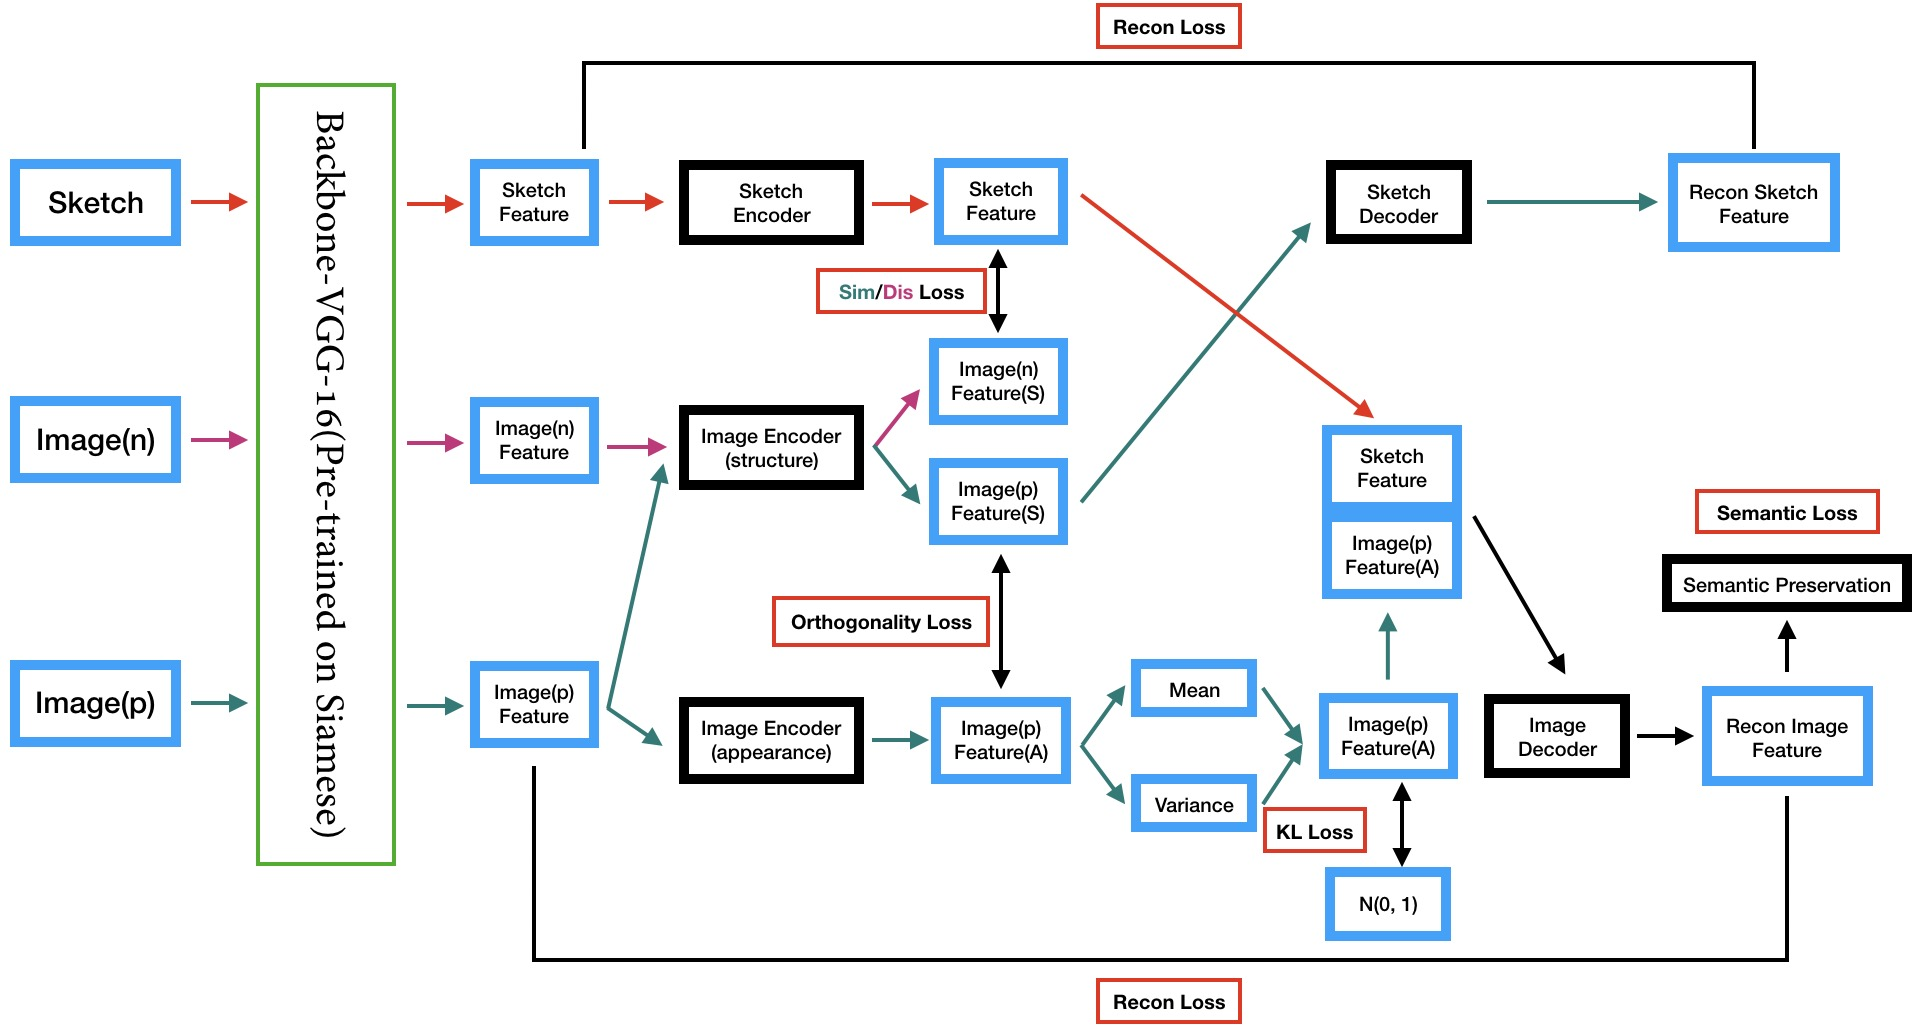
\includegraphics[width=0.95\linewidth]{model_structure.jpg}
\end{center}
   \caption{Model Structure}
\label{fig:structure}
\end{figure*}

\section{Methodology}
In this section, we introduce our proposed Bi-directional Domain Translation for zero-shot Sketch-Based Image Retrieval (BDT-SBIR) framework. In Sec \ref{3.1} we state the problem of ZS-SBIR and define some notations in this paper. In Sec \ref{3.2}, we elaborate the disentangled representation and the bi-directional translation modules in detail. In Sec \ref{3.3} we discuss the strategy during training and testing.

\subsection{Problem Definition} \label{3.1}
In this paper, we focus on solving the problem of hand-free sketch-based image retrieval under zero-shot setting, where only the sketches and images from seen categories are used during training stage. 
At the testing stage, our proposed framework is expected to use the sketches to retrieve the images, the categories of which have never appeared during training.

We first provide a definition of the SBIR in zero-shot setting. 
Given a sketch dataset $S_{sk}=\{(x_i^{sk}, y_i)|y_i \in \mathcal{Y}\}$ and an image dataset $S_{im}=\{x_j^{im}, y_j | y_j \in \mathcal{Y}\}$, where $(x_i^{sk}, y_i)$ and $(x_j^{im}, y_j)$ are corresponding to the image, sketch and their corresponding category label.
Following the zero-shot setting in \cite{yelamarthi2018zero,wang2019stacked}, we split all categories $\mathcal{Y}$ into $\mathcal{Y}_{train}$ and $\mathcal{Y}_{te}$, where no overlap exists between two label set, i.e. $\mathcal{Y}_{tr} \cap \mathcal{Y}_{te} = \emptyset$. Considering that we use ImageNet pre-trained model to extract images/sketches feature. To avoid the test category shown at training stage, we also require the testing category not in ImageNet.
Based on the partition of label set $\mathcal{Y}$, we can split sketch (resp., image) dataset into $S^{tr}_{sk}$ and $S^{te}_{sk}$ (resp., $S^{tr}_{im}$ and $S^{te}_{im}$)
%split dataset into $S^{tr}$ and $S^{te}$. 
At training stage, our model can only process the data in $S^{tr}_{sk}$ and $S_{im}^{tr}$. 
During test, given a sketch $s^{sk}$ from $S^{te}_{sk}$, our model need to retrieve images belonging to the same category as $s^{sk}$ from test images gallery $S^{te}_{im}$.

%no need to introduce the motivation in detail here. Just simply recap what you said in introduction section. Do not bring in new stuff which has not been discussed in introduction. Here, you bring in some new stuff and make our motivation harder to understand. 
%Just simplify and rewrite what we said in introduction section.

%Most of previous works maps the unaligned image and sketch pairs into a shared space and use semantic information to help the model extract semantics aligned features, whereas, the semantic information used during training is only a kind of category representation and  this kind of methods is still category-based retrieval.
%To better reduce the gap between seen categories and unseen categories, we try to factorize the image information into sketch-invariance and sketch-variance factor in latent space, which is defined as structure feature space and appearance feature space. And the disentangled information is used to match and process in different feature space respectively. 

%As illustrated in Figure \ref{fig:structure}, this is our overall end-to-end model. 
The overall framework of our method is illustrated in Figure \ref{fig:structure}.
Let $f_{im} \in \mathbb{R}^n$ be the image feature, $f_{sk} \in \mathbb{R}^n$ be the sketch feature, $f^{st}_{im} \in \mathbb{R}^m$ be the image structure feature, $f^{ap}_{im} \in \mathbb{R}^m$ be the appearance feature, $z^{ap}_{im}$ be the variational appearance feature and $f^{st}_{sk} \in \mathbb{R}^m$ be the sketch structure feature. 
Our bi-directional domain translation model builds several feature maps among these features. Before the translation, we first adopt feature extractor to map the image/sketch to their corresponding feature. Two image encoder is applied to disentangle the image feature into structure and appearance features. Meanwhile, the sketch feature is also projected into structure space. For the image-to-sketch translation, we directly use the image structure feature into the sketch space. Whereas, for the sketch-to-image translation, we combine the sketch structure feature and the image appearance feature together to get the image feature. To facilitate the stochastic sampling in retrieval, an variational estimator is adopted to image appearance feature before the combination.
%\color{red}
%Let $f_{im} \in \mathbb{R}^n$ be the image feature, $f_{sk} \in \mathbb{R}^n$ be the sketch feature, $f^{st}_{im} \in \mathbb{R}^m$ be the image structure feature, $f^{ap}_{im} \in \mathbb{R}^m$ be the appearance feature, $z^{ap}_{im}$ be the variational appearance feature and $f^{st}_{sk} \in \mathbb{R}^m$ be the sketch structure feature. 
%Our model consists of a feature extractor $F$, two structure encoders $\{E_{im}^{st}, E_{sk}\}$, one appearance encoder $\{E_{im}^{ap}\}$, one variational estimator $\{V_{im}^{ap}\}$, two domain generators $\{G_{im}, G_{sk}\}$ and two discriminators $\{D_{im}, D_{sk}\}$. 
%$F$ map image/sketch to their corresponding feature space. 
%$E_{im}^{st}$ and $E_{sk}$ map the image feature and sketch feature onto a shared structure feature space, while the $E_{im}^{ap}$ maps the image feature to the appearance feature space. $V_{im}^{ap}$ estimate the variational distribution $Q(z_{im}^{ap}|f_{im}^{ap})$, to support the variational inference during the retrieving, $G_{im}$ generates image features from encoded image structure and $G_{sk}$ generates sketch features conditional on both variational image appearance feature and encoded sketch structure. The discriminators are trained to distinguish the generated images/sketches from the real ones.

%Given these components of our model, we can define the bi-directional domain translation. The sketch to image translation is defined as $\hat{f_{img}} = G_{img}(E_{ske}(f^{ske}), V_{img}^{ap}(E_{img}^{ap}(f^{img})))$. And the image to sketch translation is defined as  $\hat{f_{ske}} = G_{ske}(E_{img}^{st}(f^{img}))$ extract the image structure features from image feature and translate them into sketch features. \color{black}
%\begin{table}[]
%\small
%\begin{tabular}{l|l}
%\hline
%Module                             & Configuration                                                               \\ \hline
%$E_{img}^{ap}$ & FC1;BatchNorm;ReLU;Dropout;FC2;BatchNorm;ReLU                               \\
%$E_{img}^{st}$ & FC1;BatchNorm;ReLU;Dropout;FC2;BatchNorm;ReLU                               \\
%$E_{ske}$                         & FC1;BatchNorm;ReLU;Dropout;FC2;BatchNorm;ReLU                               \\
%$V_{img}^{ap}$ & \begin{tabular}[c]{@{}l@{}}Mean: FC; Tanh\\ Variance: FC; Tanh\end{tabular} \\
%$G_{img}$                         & FC1;ReLU;FC2;ReLU                                                           \\
%$G_{ske}$                         & FC1;ReLU;FC2;ReLU                                                           \\
%$D_{img}$                         & FC1;BatchNorm;ReLU;Dropout;FC2;ReLU                                         \\
%$D_{ske}$                         & FC1;BatchNorm;ReLU;Dropout;FC2;ReLU                                         \\ \hline
%\end{tabular}
%\caption{The detailed configuration of our model}
%\label{table:1}
%\end{table}

\subsection{BDT-SBIR} \label{3.2}

\subsubsection{Feature Extractor} 
Since sketches are highly abstract and possess intrinsic visual sparsity compared with natural images, it is hard to extra to get more information from the pre-trained model. To alleviate this problem without adding more parameters, we use the feature fusion network in Wang el at. \cite{wang2019stacked} and concatenate the features extracted from multiple layers of the pre-trained model to get the feature of images and sketches.

In detail, we first use a pre-trained backbone model, $viz$ VGG-16 in this paper, on ImageNet \cite{deng2009imagenet} to process each sketch and image. 
Suppose $F_i \in \mathbb{R}^{C_i \times H_i \times W_i}$ is the output of the $i$-th convolution layer and $f_{fc} \in \mathbb{R}^{N}$ is the feature of the last fully connected layer, the extracted feature $f$ can be obtained by concatenating $f^{fc}$ and global average pooling (GAP) of $F^i$:

\begin{align}
f\!=\![f_{fc}, GAP(F_5), GAP(F_4), GAP(F_3)],
\end{align}
%where $GAP(\cdot)$ means global spatial average pooling and $[\cdot,\cdot, ...]$ means the concatenation operation among vectors.

\subsubsection{Disentangled Representation}
%Sketches are only outlines of images, so it is important to disentangle the $``outline"$ feature from the image feature. 
To achieve the goal of structure-based retrieval, we tend to disentangle structure information from image feature. 
We adopt two image encoder to disentangle the image feature into image structure feature and image appearance feature. Besides, to compare the image structure information with sketch in the same space, a sketch encoder is also adopt to get the sketch structure feature. 
\begin{align}
    f_{im}^{ap} \!=\! E_{im}^{ap}(f_{im}); f_{im}^{st} \!=\! E_{im}^{st}(f_{im}); f_{sk}^{st} \!=\! E_{sk}^{st}(f_{sk}).
\end{align}

At each training step, apart from sampling a positive sketch-image pair ($f_{sk}$,$f_{im^{+}}$) from the same category, we also sample another image as negative sample ($f_{im^{-}}$), which belongs to other categories. In structure feature space shared by sketch and image, we expect to pull a sketch close to the images of the same category and push a sketch apart from image of a different category. To achieve this, we design a ranking loss in structure feature space to map the disentangled image structure features to the same space as sketch structure feature. Here we use $L_2$ distance as our metric.
\begin{equation}
    \begin{aligned}
        \mathcal{L}_{rk} =& ||f_{sk}\!-\!f_{im^{\!+\!}}^{ap}||_{2}\!+\!\max(0,\!m\!-\!||f_{sk}\!-\!f_{im^{\!-\!}}^{ap}||_{2}).
    \end{aligned}
\end{equation}
Since the negative image sample is not used in the following module, we will use $f_{im}$ to represent $f_{im^{+}}$ in the following paper.

To make sure the image features are disentangled in the structure feature space and appearance feature space. 
We impose a orthogonality constrain \cite{ridgeway2018learning} that forces the structure feature and appearance feature fully disentangled.
\begin{align}
    \mathcal{L}_{or} = cos(f_{im}^{ap}, f_{im}^{sk}) = \frac{f_{im}^{ap} \bullet f_{im}^{st}}{||f_{im}^{ap}||_2 ||f_{im}^{ap}||_2}
\end{align}
Note that the $f_{img}^{ap}$ and $f_{img}^{sk}$ are the output of ReLU activation so the $cos(f_{im}^{ap}, f_{im}^{sk})$ will always more than $0$. 

%For a structure-based retrieval model, we need to align the image structure and sketch in a shared space. 
%At each training step, apart from sampling a positive sketch-image pair from the same category, we also sample another image as negative sample, which belongs to other categories. In structure feature space, we would like to reduce the distance between the positive image-sketch pair and otherwise for the negative image-sketch pair. To achieve this, we design a ranking loss in structure feature space to map the disentangled image structure features to the same space as sketch structure feature. Here we use $L_2$ distance as our metric.

\subsubsection{Bi-directional Domain Translation}
In the last part, we introduce the image-to-sketch and sketch-to-image translation, which are designed to further help the model to learn disentangled representation and take full use of the disentangled image features.

For the image-to-sketch translation, we directly use the image structure feature to reconstruct sketch feature,
\begin{align}
    \hat{f}_{sk} &= G_{sk}(f_{im}^{st}).
\end{align}
To measure the quality of the translated results,  we adopt a reconstruction loss here. To make the translated sketch feature distribution similar to the original sketch feature distribution, we also add an adversarial loss to constrain the translation results.
%\color{red}Considering the data we use in this paper is not aligned sketch-image pairs, we also add another loss to weaken constrain of the translated image/sketch, which is adversarial loss in this work,\color{black}
\begin{align}
    \mathcal{L}_{tl}^{sk} =& \log(D_{sk}(\hat{f}_{sk})) + ||f_{sk}-\hat{f}_{sk}||_2.
\end{align}

For the sketch-to-image translation, we try to use the sketch structure feature to reconstruct image feature as well. 
Whereas, considering that the images contains much more appearance information than the sketches, it is hard to compensate the appearance uncertainty from the generator only. 
Therefore, image appearance feature should be integrate to sketch structure feature. 
To facilitate the stochastic sampling, a variational estimator $V_{img}^{ap}$ is add to approximate the variational distribution $Q(z_{img}^{ap}|f_{img})$, which is assumed to be Gaussian distribution with $\mu=0$ and $\sigma=1$. The conditional distribution $P(f_{img}|z_{img}^{ap}, f_{ske}^{st})$ is modeled by a conditional generator $G_{img}$,
\begin{align}
    \mu_{im}^{ap}, \sigma_{im}^{ap} &= V_{im}^{ap}(f_{im}^{ap}), \label{eq:8} \\
    z_{im}^{ap} &= \mu_{im}^{ap} + \epsilon * \sigma_{im}^{ap} \label{eq:9} \\
    \hat{f}_{im} &= G_{im}([z_{im}^{ap}, f_{sk}^{st}])
\end{align}
where we use reparameterization trick \cite{kingma2013auto} to sample $z_{im}^{ap}$, in which $\epsilon$ is sampled from the $\mathcal{N}(0,1)$.
%the $\epsilon$ is the sampled from the $N(0,1)$ and the Equation \ref{eq:9} is the re-parameter trick.
%For the variational estimator, the evident lower bound (ELBo) is calculated from the KL-divergence between the estimated $Q(z_{img}^{ap}|f_{img})$ and hypothetical Gaussian distribution $P(z_{img}^{ap})$. 
To enforce the variational distribution $Q(z_{img}^{ap}|f_{img})$ be close to prior distribution $\mathcal{N}(0, 1)$, a Kullback-Leibler Divergence (KLD) is applied to between them. The loss function can be expressed as:
\begin{align}
    \mathcal{L}_{KL} = \!-\!D_{KL}(\mathcal{N}(\mu_{im}^{ap}, \sigma_{im}^{ap}) || \mathcal{N}(0, 1)).
\end{align}
%Note that we employ orthogonal loss on $f_{im}^{ap}$ instead of $z_{im}^{ap}$ due to the following considerations. First, we hope to used the disentangled appearance to estimate the variational feature, which can not only help our model to disentangle the image features, but also compensate the uncertain using only the appearance feature. Second, if we employ orthogonal loss in $z_{im}^{ap}$, we are indeed to make the structure feature orthogonality with normal distribution, which makes no sense.

Similar to image-to-sketch translation, the translation for sketch-to-image loss can be expressed as: 
\begin{align}
    \mathcal{L}_{tl}^{im} =& \log(D_{im}(\hat{f}_{im})) \!+\! ||f_{im}\!-\!\hat{f}_{im}||_2,
\end{align}

Besides, the discriminators are trained to distinguish the generated images/sketches from the real ones. So the loss function for discriminators are:
\begin{align}
    L_{D}^{im} &= \log(1\!-\!D_{im}(\hat{f}_{im})) \!+\! \log(D_{im}(f_{im})) \\
    L_{D}^{sk} &= \log(1\!-\!D_{sk}(\hat{f}_{sk})) \!+\! \log(D_{sk}(f_{sk}))
\end{align}

%\subsection{Cross Translation Model} \label{3.3}
%Generative approaches have shown their power in ZS-SBIR \cite{wang2019stacked,yelamarthi2018zero}. But both of these two papers, only encode the image in one encoder, which makes the appearance and the structure features fused together. When training the VAE based model, the decoder may ignore the condition information in sketch feature. Motivated by \cite{zhu2017toward}, we can regard image and sketch as two domains, where image domain have richer information than sketch domain. Our model is expected to learn a two-way mapping between this two domains. To this end, we devise a parallel VAE model, where the sketch VAE maps the image feature to the sketch domain and the image VAE maps the sketch domain to image domain with additional image appearance to complement the missing information.

%\subsubsection{Overall structure}
%In general case, a Variational Autoencoder (VAE) \cite{kingma2013auto} map a prior distribution on a hidden latent variable p(z) to the data distribution p(x). The intractable posterior p(z|x) is approximated by the variational distribution q(z|x) which is assumed to be Gaussian. In our work, the sketch VAE is expect to map the image domain to the sketch domain. The variational distribution $q(z_{i}^{ske}|f_{i}^{img})$ of the sketch VAE are estimated from $f_{img}$ via the image structure encoder $E_s^{img}$ which is a neural network parameterized by $\theta_{s}^{img}$. And the conditional $p(\hat{f}_{i}^{ske}|z_{i}^{ske})$ is modeled by the decoder network parameterized by $\phi_{skt}$. Compare with the image, the sketch are obvious lack of image information, which makes it hard to reconstruct image features from sketch only. So the variational distribution $q(z^{img}|f_{i}^{img},f_{i}^{skt})$ of the sketch VAE are estimated from both $f_{img}$ and $f_{skt}$ via the image structure encoder $E_a^{img}$ and sketch encoder $E^{ske}$ which is a neural network parameterized by $\theta_{a}^{img}$ and $\theta^{ske}$ respectively. And the conditional distribution $p(\hat{f}_{i}^{img}|z^{img}, f_{i}^{ske})$ is modeled by the decoder network parameterized by $\phi_{skt}$. 

%\subsubsection{Encoder}
%When building the image encoder and sketch encoder, both of them are excepted to receive enough information to fully represent their corresponding domain and learn some cross-modal representation between image domain and sketch domain. As we have mentioned that sketch can be regarded as the abstraction of a corresponding image.  So the sketch hidden representation is designed to be the output of the image structure encoder and the image hidden representation is designed to be the combination of the output of image appearance encoder and sketch encoder.
%In detail, the sketch and image hidden representation is formulated as :
%\begin{align}
%	z_{i}^{ske} &= E_s^{img}(f_{i}^{img}), \\
%	z_{i}^{img} &= [E_a^{img}(f_{i}^{img}), E^{skt}(f_{i}^{ske})],  \\
%\end{align}

%\subsubsection{Decoder}
%In this part, the decoders are designed to reconstruct their corresponding domain features condition on the hidden state and additional information. While, in fact, the sketch decoder is designed to make sketch hidden representation, i.e. the output of image structure encoder, more feasible to the sketch distribution. And on the other hand, the image decoder is designed to map the sketch domain to image domain for all categories including seen ones and unseen ones. So the sketch decoder is design to be a conditional decoder only condition on sketch hidden representation. For the image decoder part, the sketch feature $f_i^{ske}$ is also added to the condition.

%In detail, the reconstructed sketch and image is formulated as:
%\begin{align}
%	\hat{f}_{i}^{ske} &= D^{ske}(z_{i}^{ske}), \\
%	\hat{f}_{i}^{img} &= D^{img}(z_{i}^{img}, f_{i}^{ske}),
%\end{align}

%\subsection{Semantics Preservation} \label{3.4}
%Due to the large intra-class variance of sketches, simply using the parallel VAEs cannot overcome this. To tackle this issue, we add a semantic preserve module to ensure the image VAE to not only preserve the instance-level information with each sketch-image pair but also the category-level information of the training categories. Given the reconstructed image features $\hat{f}_{i}^{img}$, the semantics loss can be formulated as:
%\begin{align}
%	\hat{s_i} = S(\hat{f}_{i}^{img}), \\
%	\mathcal{L}^{sem} = D_{L2}(\hat{s_i}, s_i),
%\end{align}
%where the $\hat{s_i}$ is the predicted semantic representation and $s_i$ is the 

%\subsubsection{Translation Loss}
%To take full use of disentangled image representation, we first constrain the image structure features in structure feature space and use it to reconstruct the sketch feature. At the same time, we also adopt a variational estimator to image appearance feature and combine the output with sketch structure feature, which not only compensate the uncertainty during generating the image feature but also support the stochastic sampling. To this end, 

%For the image VAE and sketch VAE, the evidence lower bound (ELBo) of them are:

%\begin{equation}
%\begin{aligned}
%	&\mathcal{L}_{ske}^{ELBo}(\theta_{s}^{img}, \phi^{ske}, f_{i}^{img}, f_{i}^{ske}) = \\
%	&- D_{KL}(q(z_{i}^{ske}|f_{i}^{img})|p(z_{i}^{ske})) \\ 
%	&+ \mathbb{E}[\log p(\hat{f}_{i}^{ske}|z_{i}^{ske})]
%\end{aligned}
%\end{equation}

%\begin{equation}
%\begin{aligned}
%	&\mathcal{L}_{img}^{ELBo}(\theta_{a}^{img}, \theta^{ske}, \phi^{img}, f_{i}^{img}, f_{i}^{ske}) = \\
%	&- D_{KL}(q(z_{i}^{img}|f_{i}^{img}, f_{i}^{ske})|p(z_{i}^{img}|f_{i}^{ske})) \\
%	&+ \mathbb{E}[\log p(\hat{f}_{i}^{img}|z_{i}^{ske}, f_{i}^{ske})]
%\end{aligned}
%\end{equation}

%Furthermore, to encourage the model to preserve the latent alignments of the sketch and image, we add the reconstruction regularization to the objective:

%\begin{align}
%	\mathcal{L}_{ske}^{recon} &= D_{Euclidean}(\hat{f}_{i}^{ske}, f_{i}^{ske}) \\
%	\mathcal{L}_{img}^{recon} &= D_{Euclidean}(\hat{f}_{i}^{img}, f_{i}^{img})
%\end{align}

%\subsubsection{Orthogonality loss}
%To ensure the image structure encoder and appearance encoder different features of the image feature, we add a orthogonality loss between the output of them, which is formulated as:
%\begin{align}
%	\mathcal{L}_{\perp} = 1-D_{cosine}(E_s^{img}(f_{i}^{img}), E_{a}^{img}(f_{i}^{img}))
%\end{align}

%\subsubsection{Sketch loss}
%To better capture the sketch feature between intra-class and inner-class sketch-image pair, we add a marginal loss between positive pair ($z^{img}_{i,s}, z^{ske}_i$) and negative pair ($z^{img}_{i,s}, z^{ske}_j$), this can be formulate as:
%\begin{align}
%	Sim &= D_{L2}(E_s^{img}(f_{i}^{img}), E^{skt}(f_{i}^{ske})), \\
%	Dis &= D_{L2}(E_s^{img}(f_{j}^{img}), E^{skt}(f_{i}^{ske})), \\
%	\mathcal{L}_{dis} &= \frac{1}{2} Sim + \frac{1}{2} \max(0, m-Dis), 
%\end{align}
%where $m$ is the margin.


%So the overall loss is:
%\begin{align}
%	\mathcal{L} =& \lambda_1 \mathcal{L}_{ske}^{ELBo} + \lambda_2 \mathcal{L}_{img}^{ELBo} + \lambda_3 \mathcal{L}_{ske}^{recon} + \\ &\lambda_4 \mathcal{L}_{img}^{recon} + \lambda_5 \mathcal{L}_{\perp} + \lambda_6 \mathcal{L}_{dis} + \lambda_7 \mathcal{L}^{sem}, 
%\end{align}
%where the $\lambda_i$ are the weight for all the loss functions.

\subsection{Training and Retrieval} \label{3.3}

The full objective function can be divided into two categories, the generation loss and the discrimination loss, which can be expressed as:
\begin{align}
    \mathcal{L}_{G} \!&=\! \lambda_1 \mathcal{L}_{or} \!+\! \lambda_2 \mathcal{L}_{rk} \!+\! \lambda_3 \mathcal{L}_{KL} \!+\! \lambda_4 \mathcal{L}_{tl}^{im} \!+\! \lambda_5 \mathcal{L}_{tl}^{sk}, \\
    \mathcal{L}_{D} &= \lambda_6 L_{D}^{im} \!+\! \lambda_7 L_{D}^{sk},
\end{align}
$\lambda$ are hyper-parameters for balancing the overall performance. 
Our model consists of generators and discriminators, in order to stabilize the training process, we follow the training strategy in GAN \cite{goodfellow2014generative} to update them alternatingly with $N_{D}$ and $N_{G}$ times respectively.
%\color{red}Our model consists of generators and discriminators, so we update them alternatingly. Besides, to stabilize the training process and training the model end-to-end, we first optimize the discriminators for $D$-$iter$ times and then optimize the the translation modules for $G$-$iter$ times. The above two procedures will process in turn. \color{black}

At test stage, we divided our process into two parts.
\begin{enumerate}
    \item The image decoder is used to synthesize $N$ image features vectors $\hat{f}_{im}^{i}$ conditioned on sketch structure features and latent vector sampled from $\mathcal{N}(0,1)$. Then the average of the synthesized features is obtained to represent the final synthesized image features $\hat{f}_{im}^{re}$,
    \begin{align}
        \hat{f}_{im}^{re} = \frac{1}{n}\sum_{i=0}^{N}G_{im}([f_{sk}, z_i]),
    \end{align}
    where $z_i$ is sampled from $\mathcal{N}(0, 1)$
    \item the image structure encoder and the sketch encoder will map the images feature and sketches feature into a structure feature space as $f^{st}_{im}$ and $f^{st}_{sk}$.
\end{enumerate}

While retrieving the image, we calculate the cosine distance in structure feature space as 1-$cos(f^{st}_{im}, f^{st}_{sk})$ and that in image feature space as 1-$cos(\hat{f}_{im}^{re}, f_{im})$. Then, we use the weighted average of both as the final distance for retrieval.
\begin{equation}
\begin{aligned}
	\mathcal{D}_{fusion} =& \omega (1\!-\!cos(\hat{f}_{im}^{re}, f_{im})) +  \\
	& (1\!-\!\omega) (1\!-\!cos(f^{st}_{im}, f^{st}_{sk})), 
\end{aligned}
\end{equation}
where $\omega$ is the hyper-parameter for balancing between these two feature space.

\begin{table*}[!htb]
\resizebox{\textwidth}{!}{%
\begin{tabular}{cccccccc}
\hline \hline
                         & \multirow{2}{*}{Method} & \multicolumn{2}{c}{Sketchy Ext. (aligned)} & \multicolumn{2}{c}{Sketchy Ext. (Unaligned)} & \multicolumn{2}{c}{TU-Berlin Ext.} \\ \cline{3-8} 
                         &                         & P@200(\%)           & mAP@200(\%)          & P@200(\%)            & mAP@200(\%)           & P@200(\%)       & mAP@200(\%)      \\ \hline
\multirow{4}{*}{SBIR}    & Cosine                  & 9.0                   & 5.1                & -                      & -                   & 4.6               & 2.0            \\
                         & 3D shape \cite{wang2015sketch}               & 6.1                   & 1.0                & 7.0                    & 1.8                 & 3.6               & 0.5            \\
                         & SaN \cite{yu2017sketch}                    & 15.3                  & 5.8                & 18.9                   & 8.5                 & 10.1              & 4.2            \\
                         & Siamese \cite{yelamarthi2018zero}                & 19.3                  & 9.8               & 22.1                   & 13.9                & 8.1              & 3.7            \\ \hline
\multirow{5}{*}{ZSL}     & ESZSL \cite{romera2015embarrassingly}                  & 18.6                  & 10.0               & 18.1                   & 10.0                & 6.9               & 3.1            \\
                         & SAE  \cite{kodirov2017semantic}                   & 24.4                  & 14.4               & 27.1                   & 17.5                & 11.6              & 5.5            \\
                         & CMT \cite{socher2013zero}                    & 9.1                   & 2.2                & 8.6                    & 1.9                 & 3.8               & 0.5            \\
                         & SSE \cite{zhang2015bit}                    & 6.9                   & 2.3                & 7.3                    & 3.3                 & 4.1               & 1.2            \\
                         & DeViSE \cite{frome2013devise}                 & 9.3                   & 1.9                & 9.0                    & 1.7                 & 3.1               & 0.3            \\ \hline
\multirow{6}{*}{ZS-SBIR} & CVAE \cite{yelamarthi2018zero}                   & 33.4                  & 22.6               & 31.2                   & 19.9                & 10.2              & 4.9            \\
                         & PCYC \cite{dupont2018learning}                   & 28.0                  & 17.7               & 30.0                   & 19.4                & 12.4              & 5.7            \\
                         & Xu et al. \cite{xu2019semantic}              &                       &                    &                        &                     &                   &                \\
                         & \textbf{BDT-St}            & 37.1                  & 26.2               & 37.9                   & 26.5                & 15.2              & 7.9           \\
                         & \textbf{BDT-Im}            & 38.2                  & 27.5               & 36.1                   & 25.6                & 14.7              & 7.1           \\
                         & \textbf{BDT}            & 41.2                  & 29.9               & 39.7                   & 28.1                & 17.6              & 10.2           \\ \hline \hline
\end{tabular}%
}
\caption{ZS-SBIR performance comparison of BCD and existing methods. - means the results for the result for the two setting in Sketchy are the same. For PYCY\cite{dupont2018learning}, we remove the semantics information when training the model. For 3D shape \cite{wang2015sketch}, SaN \cite{yu2017sketch}, ESZSL \cite{romera2015embarrassingly}, SAE \cite{kodirov2017semantic}, CMT \cite{socher2013zero}, SSE \cite{zhang2015bit}, DeViSE \cite{frome2013devise} and Xu et al \cite{xu2019semantic}, we replace the semantic information with the average of image features which share the same categories\protect\footnotemark[1].}
\label{tab:1}
\end{table*}

\footnotetext[1]{We do not compare the ZSIH \cite{shen2018zero} in this table}


\section{Experiment}

\subsection{Experiment Setup}

\subsubsection{Dataset}
We evaluated BCD-SBIR on two large-scale sketch-image datasets: TU-Berlin \cite{eitz2012hdhso} and Sketchy \cite{sangkloy2016sketchy} with extended images obtained from \cite{liu2017deep}.

\textbf{Sketchy} (Extended) \cite{sangkloy2016sketchy} originally comprised 75,479 sketches and 12,500 images from 125 categories, where the image and sketch are aligned data pairs. Liu et al. \cite{liu2017deep} extended the image retrieval gallery by collecting extra 60,502 images, so that the total number of images in extended Sketchy is 73,002. Following the standard zero-shot setting in \cite{yelamarthi2018zero}, we partition the total 125 categories into 104 training categories as seen categories and 21 test categories as unseen categories according to whether the category appears in the 1,000 classes of ImageNet-1k \cite{deng2009imagenet}, which avoids violating the zero-shot assumption when utilizing models that are pre-trained on ImageNet-1k. At the training stage, there are two methods to use the training data, aligned data pair and unaligned data.

\textbf{TU-Berlin} (Extended) \cite{eitz2012hdhso} contains 250 categories with a total of 20, 000 sketches extended by \cite{liu2017deep} with natural images corresponding to the sketch classes with a total size of 204,489. Follow the same split criteria as Sketchy, we first split the TU-Berlin into 165 training categories and 85 testing categories. As the Shen et al. \cite{shen2018zero} suggest, we re-select testing categories with more than 400 images from the 85 categories. In the end, the training and testing categories of TU-Berlin are 186 and 64 respectively. Compared with Sketchy dataset, TU-Berlin is much more challenging as it contains more unseen categories and relatively less training sketches.

\subsubsection{Implementation Details}
We implement our model and all the other baseline models using the popular deep learning toolbox PyTorch \cite{paszke2017automatic}, which are all trained on one GTX 1080Ti GPU. We use a VGG-16 (pre-trained on ImageNet dataset) to extract the image and sketch features. As Sec. \ref{3.2} has mentioned, we concatenate the output of middle layers after the global average pooling (GAP) and get the 5568-D feature for each image and sketch. For each encoder, there are two fully-connected layers with Batch Normalization and ReLU activation, and one Dropout layer between them. For the variational estimator, there are two fully-connected layers working parallel to calculation the mean and the variance of the approximated $z_{im}^{ap}$ respectively. For each decoder, there are two fully-connected layers with ReLU activation. And for the discriminators, there are two fully-connected layers with Batch Normalization and LeakyReLU as activation. The dimension size for $f_{sk}^{st}$, $f_{im}^{st}$, $f_{im}^{ap}$, $z_{im}^{ap}$ are all 1024-D.

We use an Adam \cite{kingma2014adam} optimizer with learning rate of $2 \times 10^{-4}$, $\beta_1 = 0.5$, $\beta_2 = 0.999$ for optimization across our model except for the discriminators and use SGD optimizer with learning rate of $1 \times 10^{-2}$, momentum=$0.9$ for optimization across the two discriminators. The batch size for Sketchy, batch size for TU-Berlin and maximum number of training epochs are 128, 64, 30 respectively. The training iteration of generator ($N_{G}$) and discriminator ($N_{D}$) are 100 and 50 accordingly. Note that in Sketchy dataset, we perform experiments on both unaligned data and aligned data, whereas, we only use unaligned data in TU-Berlin for the lack of aligned data.

\subsection{Comparison with Existing Methods}
We compare our model with twelve prior works, which can be divided into three categories, the sketch-based image retrieval (SBIR) methods, the zero-shot learning (ZSL) methods and the zero-shot sketch-based image retrieval (ZS-SBIR) methods. 
The SBIR methods that we evaluate are Siamese \cite{yelamarthi2018zero}, SaN \cite{yu2017sketch}, 3D shape \cite{wang2015sketch} and DSH \cite{liu2017deep}. A cosine baseline is also added, which compute the 4096-D VGG-16 \cite{simonyan2014very} feature vector pre-trained on ImageNet-1k for nearest neighbor search.
The ZSL methods that we evaluate are ESZSL \cite{romera2015embarrassingly}, SAE \cite{kodirov2017semantic}, CMT \cite{socher2013zero}, SSE \cite{zhang2015bit} and DeViSE \cite{frome2013devise}.
The ZS-SBIR methods that we evaluate are CVAE \cite{yelamarthi2018zero}, PCYC \cite{dutta2019semantically} and Xu et al. \cite{xu2019semantic}.
For fair comparison, we replace the backbone of all the previous model to VGG-16, except for the SaN, which propose a new backbone to extract information from sketch and image. 
All the backbones are pre-trained on ImageNet-1k. 
Since we do not use additional semantic information obtained from large textual corpus (e.g., word vector \cite{mikolov2013distributed} and WordNet \cite{miller1998wordnet}) in our model, we also remove the semantics information or replace the semantics information to the average of image features, which share the same category, for all the baselines. 
Besides, we do not compare with the methods that need to fine-tune the pre-trained backbone during training the retrieval model, like SAKE \cite{liu2019semantic} and EMS \cite{lu2018learning}. 
We use mean average precision and precision considering top 200 (mAP@200 and P@200) retrievals for evaluation and comparison.


Table \ref{tab:1} shows the results of our proposed BDT and all the comparison methods. 
From the results, we can find that most of the SBIR and ZSL methods perform worse than the ZS-SBIR methods. 
Compare with the results of Cosine, the 3D shape \cite{wang2015sketch}, CMT \cite{socher2013zero}, SSE \cite{zhang2015bit} and the DeViSE \cite{frome2013devise} perform ever worse, which indicates these model are prone to overfit in seen category. 
In Sketchy Ext. dataset, we find the model train on the unaligned data usually perform better than the aligned data, which mainly because that the number of unaligned data are five times more than that of aligned data and large training data can help the model better generalize from seen to unseen categories. 
Whereas, CVAE shows the opposite tendency, as in this case, the aligned data with pose similarity can help the model learn structure-based retrieval when reconstruct the image from the sketch. 
For the TU-Berlin Ext. dataset, the number of the unseen categories under our split are two times more than that in prior works \cite{liu2019semantic, dutta2019semantically} and our split also guarantee that there is not information leak from unseen categories, so that the results in our paper is much more lower than that in prior works \cite{liu2019semantic, dutta2019semantically}.

Our proposed BDT has excelled the state-of-the-art methods by 7.8\% P@200 in Sketchy Ext. (aligned) dataset, 8.5\% P@200 in Sketchy Ext. (unaligned) dataset and 5.2\% P@200 in TU-Berlin Ext. dataset. 
To better realize the advantage of our proposed method, we also list the retrieval results from only the image feature space and the structure space as \textbf{BDT-Im} and \textbf{BDT-St}. Compare the results between \textbf{BDT-Im} and CVAE and the results between \textbf{BDT-St} and Siamese, the disentangled representation is indeed help the model to generalize from seen to unseen categories. 
Besides, the results among \textbf{BDT-Im}, \textbf{BDT-St} and \textbf{BDT} show that retrieval from both image feature space and structure feature space can boosting the result by a large margin, which also indicates that retrieval results of these two space can compensate each other.

\begin{table}[]
\resizebox{0.47\textwidth}{!}{%
\begin{tabular}{lcccc}
\hline \hline
 & \multicolumn{2}{c}{Sketchy Ext. (aligned)} & \multicolumn{2}{c}{Sketchy Ext. (unaligned)} \\ \cline{2-5} 
\multicolumn{1}{c}{} & P@200(\%) & mAP@200(\%) & P@200(\%) & mAP@200(\%) \\ \hline
-$L_{rk}$ & 35.1 & 23.2 & 31.7 & 20.3 \\
-$L_{or}$ & 40.3 & 29.1 & 38.4 & 26.9 \\
-$L_{recog}^{im}$ & 31.7 & 19.8 & 32.1 & 20.5 \\
-$L_{recog}^{sk}$ & 39.9 & 28.3 & 38.3 & 27.8 \\
-$L_{adv}^{im}$ & 40.0 & 28.3 & 35.5 & 24.9 \\
-$L_{adv}^{sk}$ & 40.7 & 29.6 & 39.3 & 27.9 \\
moved $L_{or}$ & 39.1 & 27.4 & 37.9 & 26.6 \\
sk2im & 37.2 & 26.0 & 36.5 & 25.9 \\ \hline \hline
\end{tabular}%
}
\caption{Ablation Study on Sketchy Ext. moved $\mathcal{L}_{or}$ means that we move the orthogonality loss from ($f_{im}^{ap},f_{im}^{st}$) to ($z_{im}^{ap},f_{im}^{st}$); sk2im means we directly translate the image from the sketch structure feature and ignore the variational estimator.}
\label{tab:2}
\end{table}

\subsection{Ablation Study}
We analyze the effect of different loss function, some alternations while designing the model and the effect of $\omega$ on Sketchy Ext dataset.

\noindent\textbf{Loss Analysis}
In Table \ref{tab:2}, we can find the effect of different losses. As expected, the ranking loss and the image reconstruction loss are the most important constrain in our model, which is because these two losses mainly control the image-sketch distance in their corresponding space. Besides, the image reconstruction loss has bigger effect on aligned data than that on unaligned data, which indicated the reconstruction loss is sensitive to the pose information. The image adversarial loss have much bigger effect on the unaligned dataset, which shows the adversarial loss can relief the strong constrain bring from image reconstruction loss in unaligned data. 

\noindent\textbf{Alternation Analysis}
In the last two rows, we show two alternations, (1) move the orthogonality loss from ($f_{im}^{ap},f_{im}^{st}$) to ($z_{im}^{ap},f_{im}^{st}$) and (2) directly translate the image from the sketch structure feature and ignore the variational estimator. The performance drop after moving the orthogonality loss to $z_{im}^{ap}$ and $f_{im}^{st}$ indicate the effect of the disentangled representation. And the performance drop after we remove the variational estimator indicates the uncertainty image appearance compensate is crucial to train the image generator.

\noindent\textbf{Retrieval Strategy  Analysis}
In Figure \ref{fig:omega}

\subsection{Case study}

\section{Conclusion}

\section{Comments}
\begin{itemize}
	\item Abs the zs-sbir is introduced in second and third sentences
	\item name of the model
	\item disentangled representation
\end{itemize}


{\small
\bibliographystyle{ieee_fullname}
\bibliography{egbib}
}

\end{document}
